%%%%%%%%%%%%%%%%%%%%%%%%%%%%%%%%%%%%%%%%%%%%%%%%%%%%%%%%%%%%%%%%%%%%%%%%%%%%%%%%%%
\begin{frame}[fragile]\frametitle{}
\begin{center}
{\Large K-Means with Scikit-Learn}
\end{center}
\end{frame}


%%%%%%%%%%%%%%%%%%%%%%%%%%%%%%%%%%%%%%%%%%%%%%%%%%%%%%%%%%%%%%%%%%%%%%%%
\begin{frame}[fragile]\frametitle{K-Means}
\begin{lstlisting}
from sklearn import datasets
from sklearn.cluster import KMeans
import matplotlib.pyplot as plt
from mpl_toolkits.mplot3d import Axes3D

# load the iris datasets
dataset = datasets.load_iris()
X = iris.data
# fit a K-means to the data
km = KMeans(n_clusters=3)
km.fit(X)
km.predict(X)
labels = km.labels_
fig = plt.figure(1, figsize=(7,7))
ax = Axes3D(fig, rect=[0, 0, 0.95, 1], elev=48, azim=134)
ax.scatter(X[:, 3], X[:, 0], X[:, 2],
          c=labels.astype(np.float), edgecolor="k", s=50)
ax.set_xlabel("Petal width")
ax.set_ylabel("Sepal length")
ax.set_zlabel("Petal length")
plt.title("K Means", fontsize=14)
\end{lstlisting}

{\tiny (Ref: Clustering Based Unsupervised Learning - Syed Sadat Nazrul)}

\end{frame}

%%%%%%%%%%%%%%%%%%%%%%%%%%%%%%%%%%%%%%%%%%%%%%%%%%%%%%%%%%%%%%%%%%%%%%%%
\begin{frame}[fragile]\frametitle{K-Means Plotting}
\begin{center}
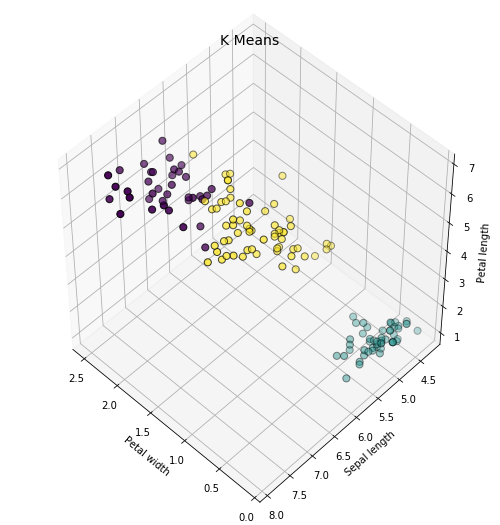
\includegraphics[width=0.6\linewidth,keepaspectratio]{kmeans1}
\end{center}

{\tiny (Ref: Clustering Based Unsupervised Learning - Syed Sadat Nazrul)}

\end{frame}

% %%%%%%%%%%%%%%%%%%%%%%%%%%%%%%%%%%%%%%%%%%%%%%%%%%%%%%%%%%%
% \begin{frame}[fragile]\frametitle{K-Means Sklearn Template Code}
% \begin{lstlisting}
% from sklearn.cluster import KMeans 

% #Assumed you have, X (attributes) for training data set and x_test(attributes) of test_dataset 

% k_means = KMeans(n_clusters=3, random_state=0) 

% model.fit(X) 

% predicted= model.predict(x_test) 
% \end{lstlisting}
% \end{frame}

% %%%%%%%%%%%%%%%%%%%%%%%%%%%%%%%%%%%%%%%%%%%%%%%%%%%%%%%%%%%%%%%%%%%%%%%%%%%%%%%%%%
% \begin{frame}[fragile]\frametitle{}
% \begin{center}
% {\Large Test case: UN data}
% \end{center}
% \end{frame}

% %%%%%%%%%%%%%%%%%%%%%%%%%%%%%%%%%%%%%%%%%%%%%%%%%%%%%%%%%%%
% \begin{frame}[fragile]\frametitle{K-Means Example: UN data}
% \begin{lstlisting}
% # load the UN data-set transformed to float with 4 columns, 
% # lifeMale,lifeFemale,infantMortality and GDPperCapita

% fName = ('../datasets/UN4col.csv')
% fp = open(fName)
% X = np.loadtxt(fp)
% fp.close()

% from sklearn.cluster import KMeans
% km = KMeans(3, init='k-means++') 
% km.fit(X)
% c = km.predict(X) 
% \end{lstlisting}
% \end{frame}

% %%%%%%%%%%%%%%%%%%%%%%%%%%%%%%%%%%%%%%%%%%%%%%%%%%%%%%%%%%%
% \begin{frame}[fragile]\frametitle{K-Means Example: Plot}
% \begin{lstlisting}
% import matplotlib.pyplot as plt
% def plot_clusters(orig,pred,nx,ny):
	% data = orig
	% ylabels = { 0:'Male life expectancy in yrs',1:'Female life expectancy in yrs',2:'Infant mortality, per 1000'}

	% p0 = plt.plot(data[pred==0,nx],data[pred==0,ny],'ro',label='Underdeveloped')
	% p2 = plt.plot(data[pred==2,nx],data[pred==2,ny],'go',label='Developing') 
	% p1 = plt.plot(data[pred==1,nx],data[pred==1,ny],'bo',label='Developed') 

	% lx = p1[0].axes.set_xlabel('Per Capita GDP in US$')
	% ly = p1[0].axes.set_ylabel(ylabels[ny])
	% tt= plt.title('UN countries Dataset, K=3')
  % return (p0,p1,p2)
% \end{lstlisting}
% % % (Ref: github.com/nborwankar/LearnDataScience/\ldots/kmeans.py)
% \end{frame}


% %%%%%%%%%%%%%%%%%%%%%%%%%%%%%%%%%%%%%%%%%%%%%%%%%%%%%%%%%%%
% \begin{frame}[fragile]\frametitle{K-Means Example: Plot}
% \begin{lstlisting}
% (pl0,pl1,pl2) = plot_clusters(X,c,3,2) # column 3 GDP, vs column 2 infant mortality. Note indexing is 0 based
% \end{lstlisting}
% \begin{center}
% 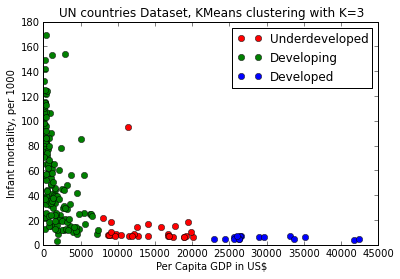
\includegraphics[width=0.6\linewidth,keepaspectratio]{clust1}
% \end{center}
% \end{frame}
% %%%%%%%%%%%%%%%%%%%%%%%%%%%%%%%%%%%%%%%%%%%%%%%%%%%%%%%%%%%
% \begin{frame}[fragile]\frametitle{K-Means Example: Plot}
% \begin{lstlisting}
% (pl0,pl1,pl2) = plot_clusters(X,c,3,0,False)
% \end{lstlisting}
% \begin{center}
% 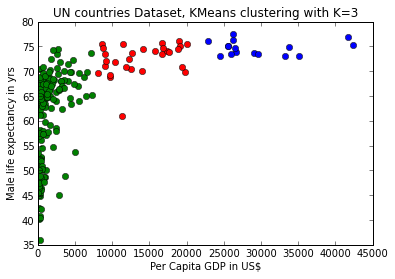
\includegraphics[width=0.6\linewidth,keepaspectratio]{clust2}
% \end{center}
% \end{frame}

% %%%%%%%%%%%%%%%%%%%%%%%%%%%%%%%%%%%%%%%%%%%%%%%%%%%%%%%%%%%
% \begin{frame}[fragile]\frametitle{K-Means Example: Plot}
% \begin{lstlisting}
% (pl0,pl1,pl2) = plot_clusters(X,c,3,1,False)
% \end{lstlisting}
% \begin{center}
% 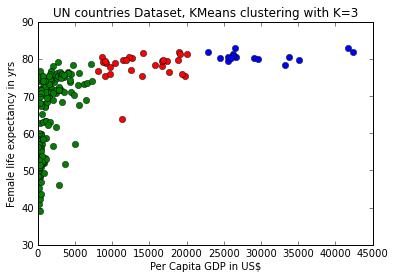
\includegraphics[width=0.6\linewidth,keepaspectratio]{clust3}
% \end{center}
% \end{frame}

% %%%%%%%%%%%%%%%%%%%%%%%%%%%%%%%%%%%%%%%%%%%%%%%%%%%%%%%%%%%%%%%%%%%%%%%%%%%%%%%%%%
% \begin{frame}[fragile]\frametitle{}
% \begin{center}
% {\Large Test case: Beer}
% \end{center}
% \end{frame}


% %%%%%%%%%%%%%%%%%%%%%%%%%%%%%%%%%%%%%%%%%%%%%%%%%%%%%%%%%%%
% \begin{frame}[fragile]\frametitle{K-Means Example: Beer data}
% \begin{lstlisting}
% import pandas as pd
% url = 'https://raw.githubusercontent.com/justmarkham/DAT8/master/data/beer.txt'
% beer = pd.read_csv(url, sep=' ')
% \end{lstlisting}
% \begin{center}
% 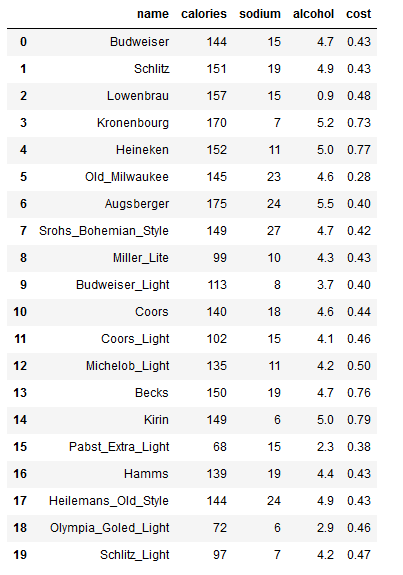
\includegraphics[width=0.3\linewidth,keepaspectratio]{clust4}
% \end{center}
% How would you cluster these beers?
% \end{frame}


% %%%%%%%%%%%%%%%%%%%%%%%%%%%%%%%%%%%%%%%%%%%%%%%%%%%%%%%%%%%
% \begin{frame}[fragile]\frametitle{K-Means Example: Clustering}
% \begin{lstlisting}
% X = beer.drop('name', axis=1)

% from sklearn.cluster import KMeans

% km = KMeans(n_clusters=3, random_state=1)
% km.fit(X)

% print(km.labels_)
% # array([0, 0, 0, 0, 0, 0, 0, 0, 1, 1, 0, 1, 0, 0, 0, 2, 0, 0, 2, 1])

% # save the cluster labels and sort by cluster
% beer['cluster'] = km.labels_
% beer.sort('cluster')
% \end{lstlisting}
% What do the clusters seem to be based on? Why?
% \end{frame}

% %%%%%%%%%%%%%%%%%%%%%%%%%%%%%%%%%%%%%%%%%%%%%%%%%%%%%%%%%%%
% \begin{frame}[fragile]\frametitle{K-Means Example: Review Clusters}
% \begin{lstlisting}
% print(km.cluster_centers_)
% array([[ 150., 17., 4.52142857,0.52071429],
       % [ 102.75,10., 4.075,0.44 ],
       % [  70,10.5,2.6,0.42]])
% beer.groupby('cluster').mean()
% centers = beer.groupby('cluster').mean()
% \end{lstlisting}
% \begin{center}
% 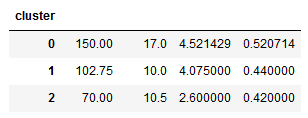
\includegraphics[width=0.5\linewidth,keepaspectratio]{clust5}
% \end{center}
% \end{frame}

% %%%%%%%%%%%%%%%%%%%%%%%%%%%%%%%%%%%%%%%%%%%%%%%%%%%%%%%%%%%
% \begin{frame}[fragile]\frametitle{K-Means Example: Plotting}
% \begin{lstlisting}
% import matplotlib.pyplot as plt
% import numpy as np

% plt.rcParams['font.size'] = 14
% colors = np.array(['red', 'green', 'blue', 'yellow'])
% plt.scatter(beer.calories, beer.alcohol, 
			% c=colors[beer.cluster], s=50)
% plt.scatter(centers.calories, centers.alcohol,
			% linewidths=3, marker='+', s=300, c='black')
% plt.xlabel('calories')
% plt.ylabel('alcohol')
% \end{lstlisting}
% \begin{center}
% 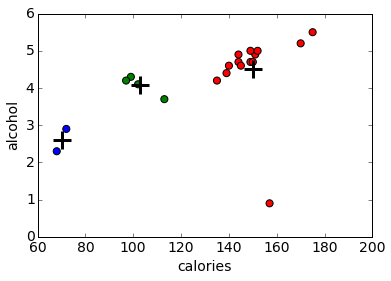
\includegraphics[width=0.35\linewidth,keepaspectratio]{clust6}
% \end{center}
% \end{frame}

% %%%%%%%%%%%%%%%%%%%%%%%%%%%%%%%%%%%%%%%%%%%%%%%%%%%%%%%%%%
% \begin{frame}[fragile]\frametitle{K-means Algorithm (recap)}
% \begin{itemize}
% \item  K-means is an iterative, unsupervised clustering algorithm that groups similar instances together into clusters. 
% \item The algorithm starts by guessing the initial centroids for each cluster
% \item Then repeatedly assigns instances to the nearest cluster and re-computes the centroids of that clusters. 
% \end{itemize}
% \end{frame}


